% Slides for talk on hydrogen fuel cells
% given in the department on October 27, 2003.
% 
% The original slides were in Prosper.  This file contains the
% translation of the original slides to Beamer.% 
% Rouben Rostamian <rostamian@umbc.edu>
% August 31, 2004

\documentclass[10pt]{beamer}
%\usetheme{umbc4}
\usetheme{Boadilla}
\useinnertheme{umbcboxes}
\setbeamercolor{umbcboxes}{bg=violet!12,fg=black}
\def\newblock{\hskip .11em plus .33em minus .07em}

\setbeamertemplate{navigation symbols}{}

\usepackage{rotating} % for defining \schwa
\usepackage{amsmath}
\usepackage{subfigure}
\usepackage{bm}
\usepackage{natbib}
\usepackage{hyperref}
\usepackage{soul}

\newcommand{\apj}{ApJ}
\newcommand{\apjl}{ApJL}
\newcommand{\mnras}{MNRAS}
\newcommand{\aap}{A\&A}
\newcommand{\pasj}{PASJ}
\newcommand{\araa}{ARAA}
\newcommand{\C}{\mathcal{C}^\lambda}
\newcommand{\real}{\operatorname{Re}}
\newcommand{\ii}{\mathrm{i}}
\newcommand{\schwa}{\raisebox{1ex}{\begin{turn}{180}e\end{turn}}}
\newcommand{\imag}{\operatorname{Im}}


\newcommand{\arcsinh}{\mathop\mathrm{arcsinh}\nolimits}
\newcommand{\arccosh}{\mathop\mathrm{arccosh}\nolimits}
\newcommand{\Pu}{P_{\mathrm{amb}}}
\newcommand{\adot}{\dot{a}}
\newcommand{\p}{\partial}
\newcommand{\dd}{\delta}
\newcommand{\sbar}{\bar{\sigma}}

\title[Disk instabilities]{Instabilities in protoplanetary disks and
  its role in planet formation} 
\author[M-K. Lin]{Min-Kai Lin\\mklin924@cita.utoronto.ca}
\institute[CITA]{ Canadian Institute for Theoretical Astrophysics}
\date{October 1 2013}
\begin{document}

\begin{frame}[plain]
  \titlepage
\end{frame}


\begin{frame}
   \frametitle{Sub-structures in protoplanetary disks}
   \centering
   \begin{figure}
     \includegraphics[width=0.6\linewidth]{spiral.jpg}
   \end{figure} 
   (Grady et al. 2013)
\end{frame}

\begin{frame}
   \frametitle{Large-scale hydrodynamic instabilities}
    \centering
    \begin{onlinebox}{9cm} Gravitational instability
      of dead zone boundaries\end{onlinebox}
   \begin{figure}
%   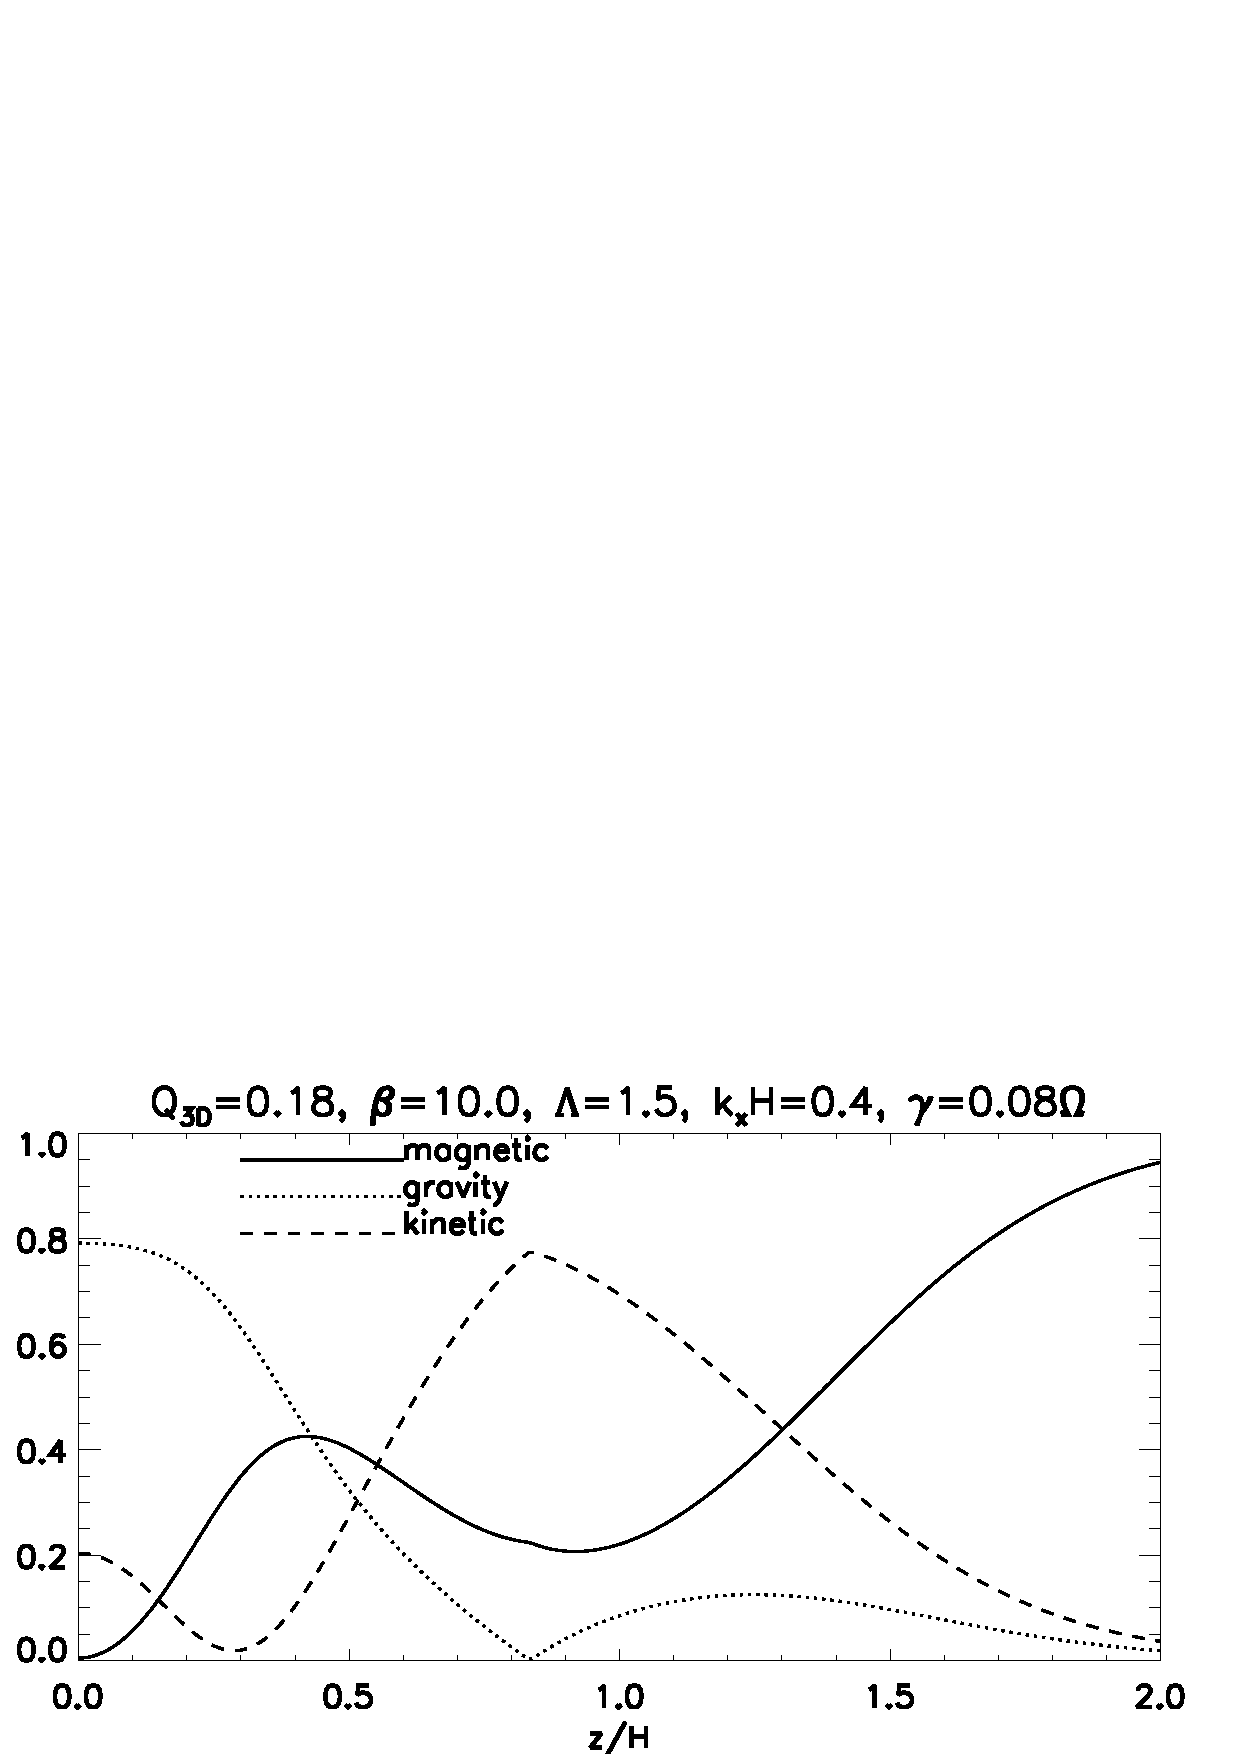
\includegraphics[scale=0.55,clip=true, trim=0cm 0cm 1.45cm
%   16.43cm]{result.pdf}
     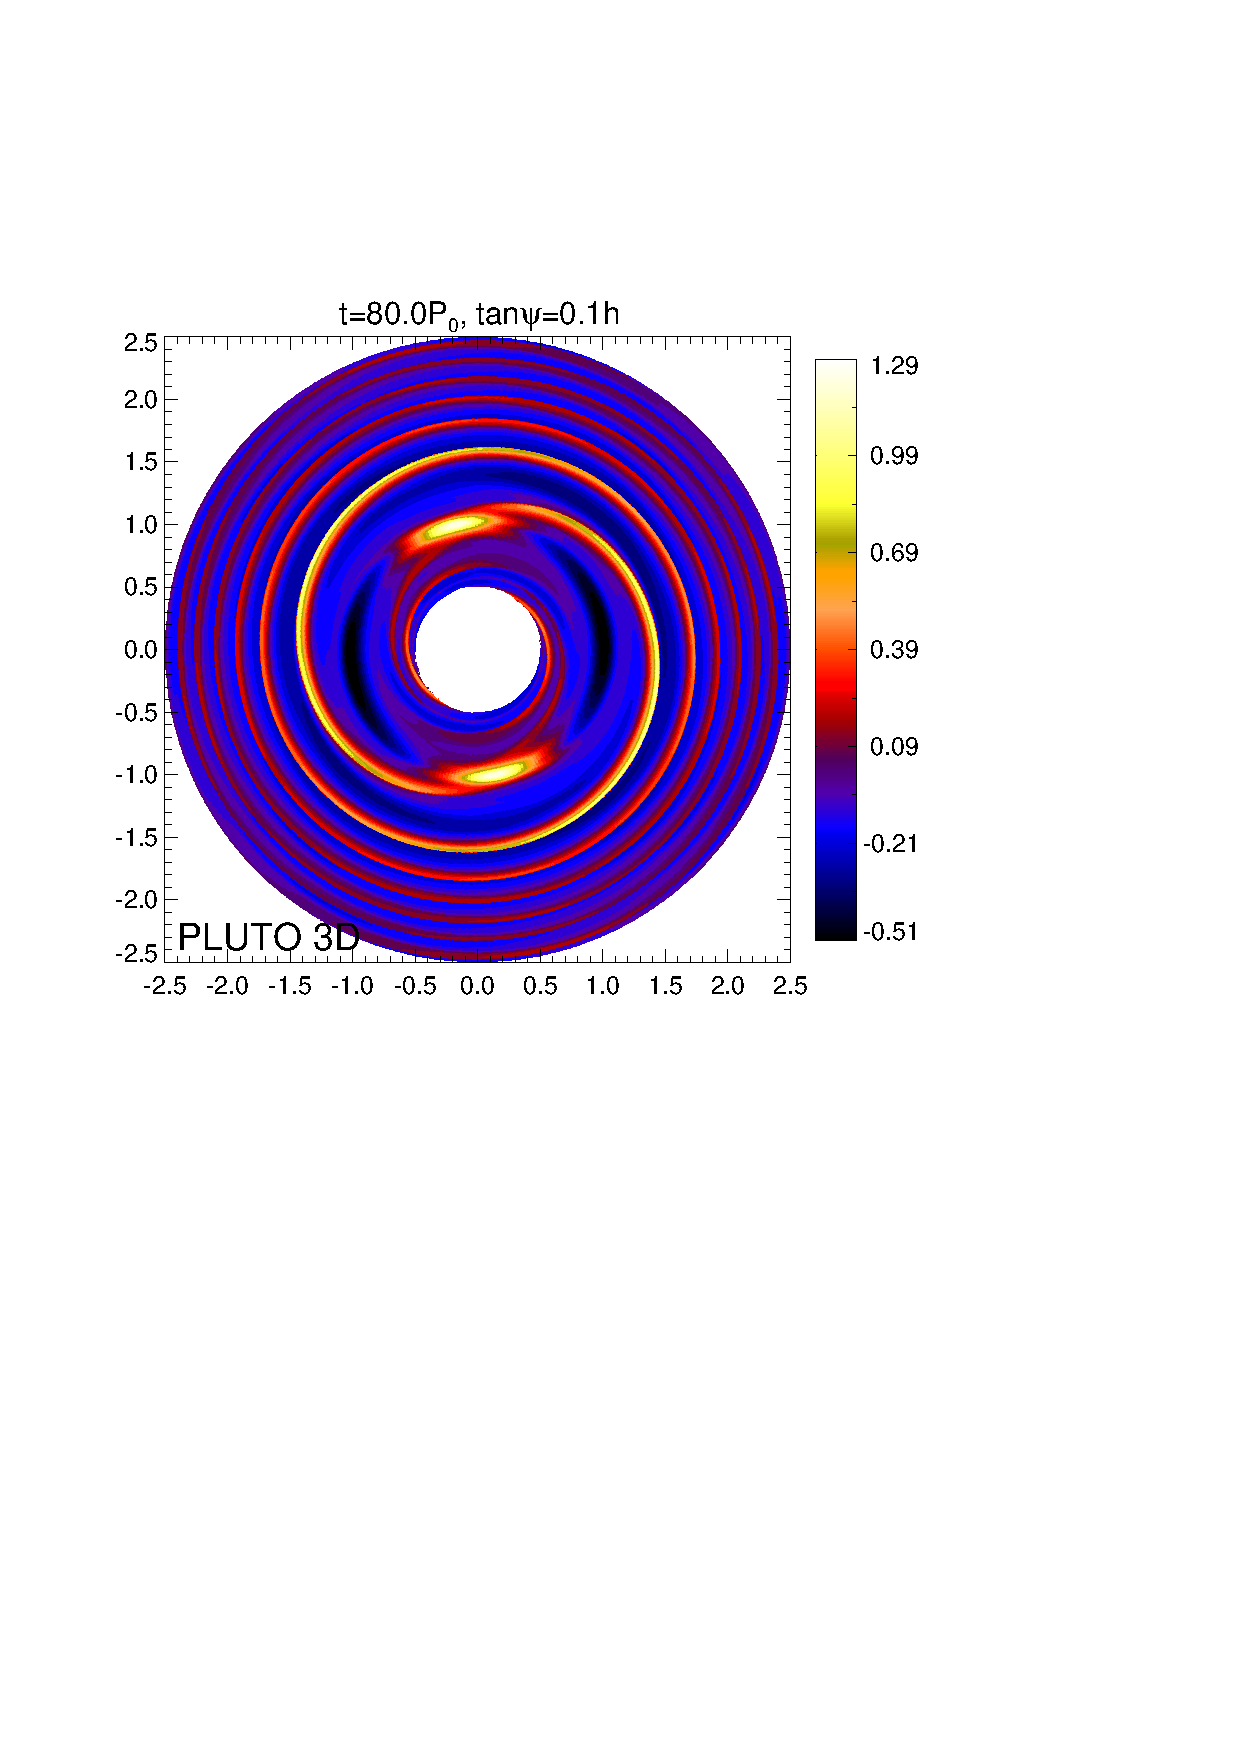
\includegraphics[width=0.48\linewidth,clip=true,trim=1.9cm
       12.75cm 5.9cm 3.3cm]{pdiskxy_008.pdf}\includegraphics[width=0.48\linewidth,clip=true,trim=1.9cm
       12.75cm 5.9cm 3.3cm]{polarxy2_dens008.pdf}
   \end{figure} 
   Astrophysical fluid codes: FARGO, ZEUS, PLUTO , (ATHENA)
\end{frame}

\begin{frame}[t]
  \frametitle{Linear hydrodynamics}
  \centering
    \begin{onlinebox}{9cm}Resistive magneto-rotational instability in
      massive disks\end{onlinebox}
   \begin{figure}
   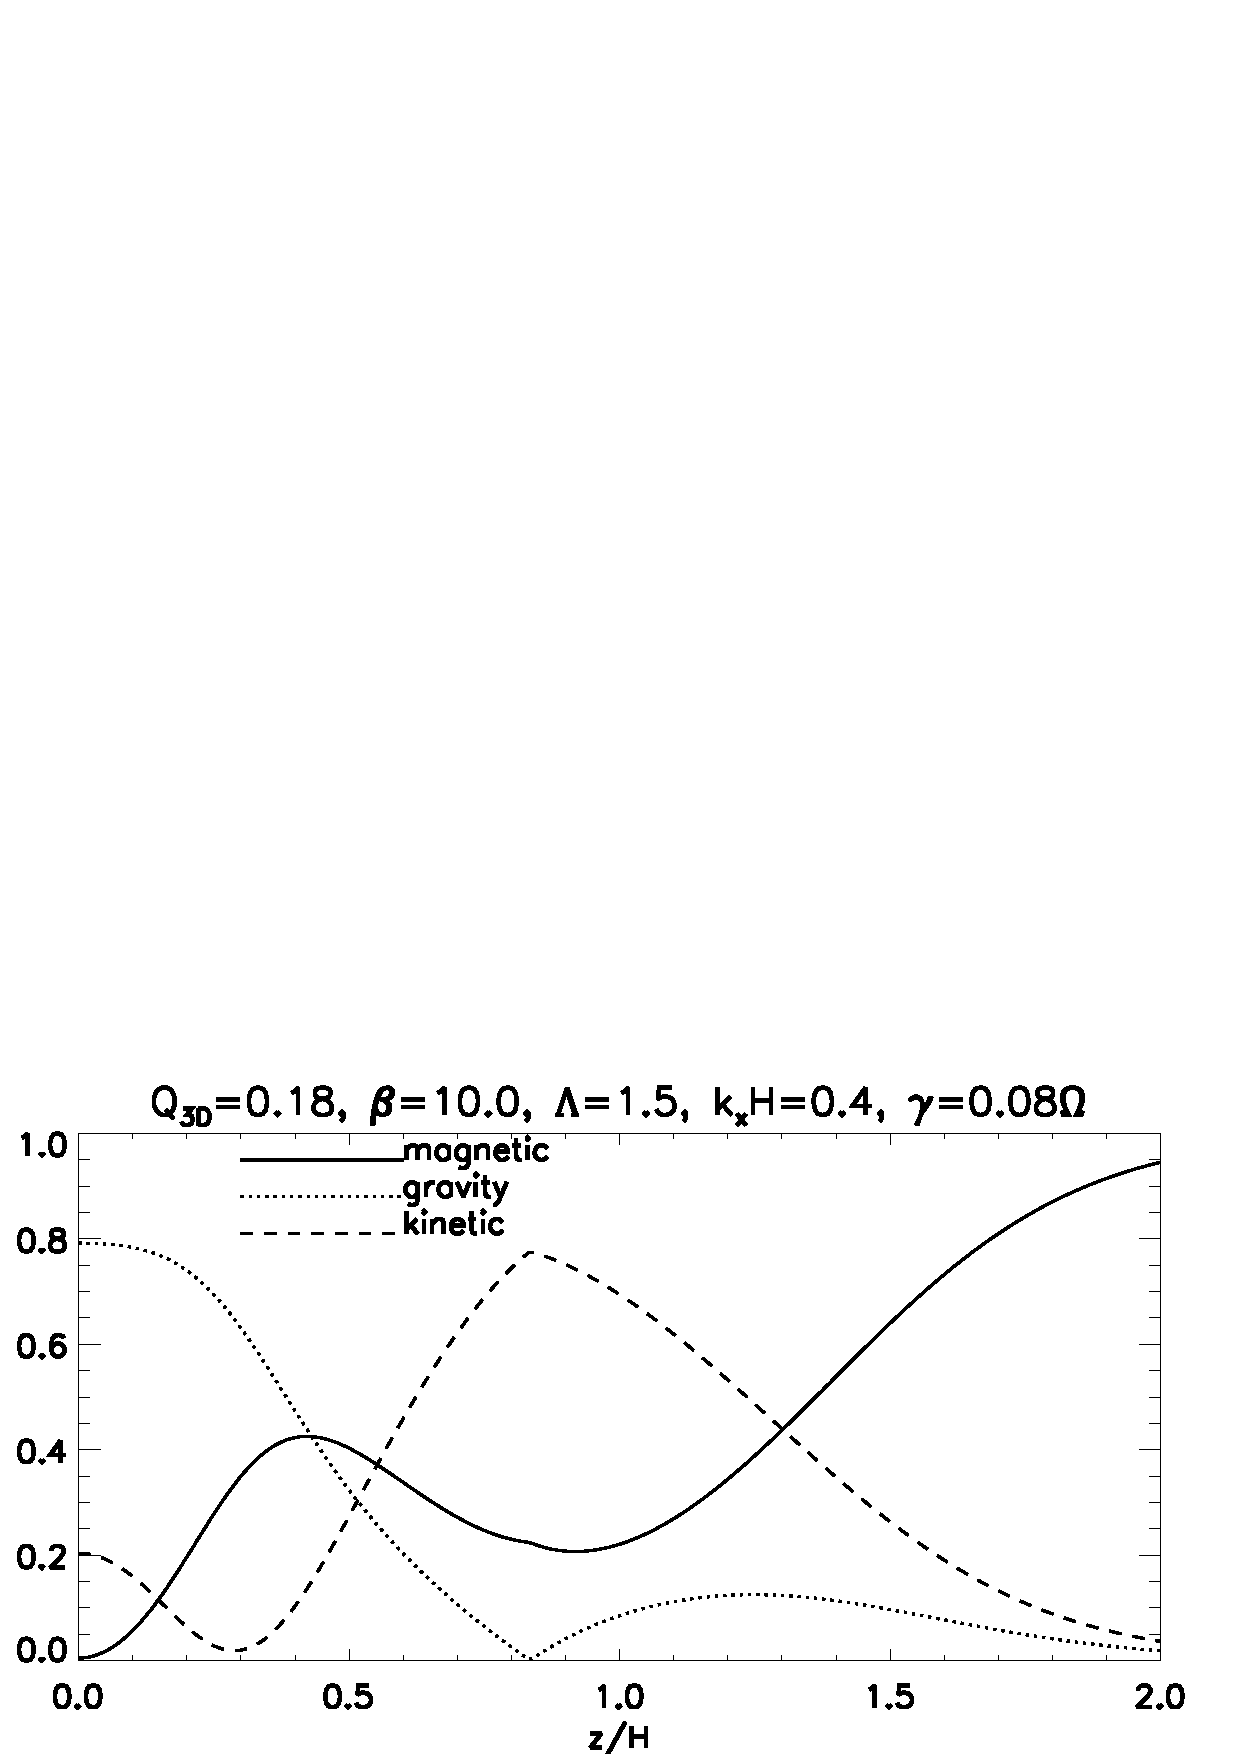
\includegraphics[scale=0.55,clip=true, trim=0cm 0cm 1.45cm 16.43cm]{result.pdf}
%   \includegraphics[scale=.5]{result.ps}
   \end{figure} 
  
(Lin and Menou, in prep.) 
\end{frame}

\end{document}
